\section{The entropy law}\label{sec:entropy}

\subsection{Two inequalities}

Everything in this section rests on $\log x\le x-1$ for $x>0$, with equality only at $x=1$.

\begin{lemma}[Gibbs term]\label{lem:gibbs}
For $x,y>0$, $x\log(1/x)\le x\log(1/y)+y-x$, with equality if and only if $x=y$.
\end{lemma}

\begin{proof}
Apply $\log t\le t-1$ to $t=y/x$ and multiply by $x$: $x\log y-x\log x\le y-x$.
\end{proof}

\begin{lemma}[Entropy term]\label{lem:entropyterm}
For $a,b,A,\theta>0$,
\[
a\log\frac Aa+a\log\frac1\theta\ \le\ a\log\frac1b+\frac{Ab}{\theta}-a,
\]
with equality if and only if $b=\theta a/A$.
\end{lemma}

\begin{proof}
Apply $\log t\le t-1$ to $t=Ab/(\theta a)$, so that $\log A+\log b-\log\theta-\log a\le Ab/(\theta a)-1$, and multiply by $a$.
\end{proof}

\begin{proposition}[Entropy inequality]\label{prop:entropyineq}
Let $a_{1},\dots,a_{n}>0$ with sum $A$, let $\beta_{1},\dots,\beta_{n}>0$ and $\theta>0$ with $\sum_{i}\beta_{i}\le\theta$. Then
\begin{equation}\label{eq:entropyineq}
A\,H(p)+A\log\frac1\theta\ \le\ \sum_{i}a_{i}\log\frac1{\beta_{i}},
\end{equation}
with equality if and only if $\beta_{i}=\theta p_{i}$ for every $i$.
\end{proposition}

\begin{proof}
Sum Lemma~\ref{lem:entropyterm} with $(a,b)=(a_{i},\beta_{i})$. By \eqref{eq:AH} the left side is $AH(p)+A\log(1/\theta)$, and the right side is $\sum_{i}a_{i}\log(1/\beta_{i})+(A/\theta)\sum_{i}\beta_{i}-A\le\sum_{i}a_{i}\log(1/\beta_{i})$. Equality forces equality in every term and $\sum_{i}\beta_{i}=\theta$, that is $\beta_{i}=\theta a_{i}/A$.
\end{proof}

The inequality says that among all ways of spending a budget $\theta$ of false acceptances on $n$ items, the weighted sum of the ``surprisals'' $\log(1/\beta_{i})$ is least when the budget is shared in proportion to the costs. It is Gibbs' inequality for the probability vectors $p$ and $\beta/\theta$, with a slack $\theta-\sum\beta_{i}$ that only helps.

\subsection{Proof of the entropy law}

\begin{proof}[Proof of Theorem~\ref{thm:A}]
We treat finitely many candidates; the infinite case is Proposition~\ref{prop:infinite}.

\emph{Lower bound.} Let $r$ satisfy $\sum_{i}\eps^{r_{i}}\le\theta$ and put $\beta_{i}=\eps^{r_{i}}>0$. Then $\log(1/\beta_{i})=r_{i}L$, and Proposition~\ref{prop:entropyineq} gives
\[
AH(p)+A\log\frac1\theta\ \le\ L\sum_{i}a_{i}r_{i}=L\,V(r).
\]
Dividing by $L$ and taking the minimum over $r$ gives the left inequality of \eqref{eq:entropylaw}.

\emph{Upper bound.} Let $r_{i}=\lceil x_{i}\rceil$ with $x_{i}=\log(A/(\theta a_{i}))/L$. Since $\theta\le1$ and $a_{i}\le A$, $x_{i}\ge0$, so $x_{i}\le r_{i}<x_{i}+1$. The first inequality gives $\eps^{r_{i}}\le\eps^{x_{i}}=\theta a_{i}/A$, hence $\sum_{i}\eps^{r_{i}}\le\theta$. The second gives
\[
V(r)<\sum_{i}a_{i}\Bigl(\frac1L\log\frac{A}{\theta a_{i}}+1\Bigr)=\frac AL\Bigl(H(p)+\log\frac1\theta\Bigr)+A .
\]

\emph{Equality.} If $\theta p_{i}=\eps^{k_{i}}$ with $k_{i}\in\NN$, the schedule $r_{i}=k_{i}$ has $\sum\eps^{r_{i}}=\theta\sum p_{i}=\theta$ and $V(r)=\sum_{i}a_{i}\log(1/(\theta p_{i}))/L=(A/L)(H(p)+\log(1/\theta))$.

\emph{The constant $A$.} Take $\eps=\frac12$, $\theta=1$, $n=2$ and $a=(1-t,t)$ with $0<t<\frac12$. A schedule with $r_{1}=0$ or $r_{2}=0$ has $\sum2^{-r_{i}}>1$, so every feasible schedule has $r_{1},r_{2}\ge1$, and $r=(1,1)$ is feasible; hence $\Vs(1)=A=1$. The lower bound is $H(p)/\log2$, which tends to $0$ as $t\to0$. So the gap $\Vs-(A/L)(H+\log\frac1\theta)$ approaches $A$, and no constant $cA$ with $c<1$ bounds it.
\end{proof}

Figure~\ref{fig:schedule} shows the ceiling schedule for a power-law profile and compares its cost with the lower bound over twelve decades of $\theta$.

\begin{figure*}[t]
\centering
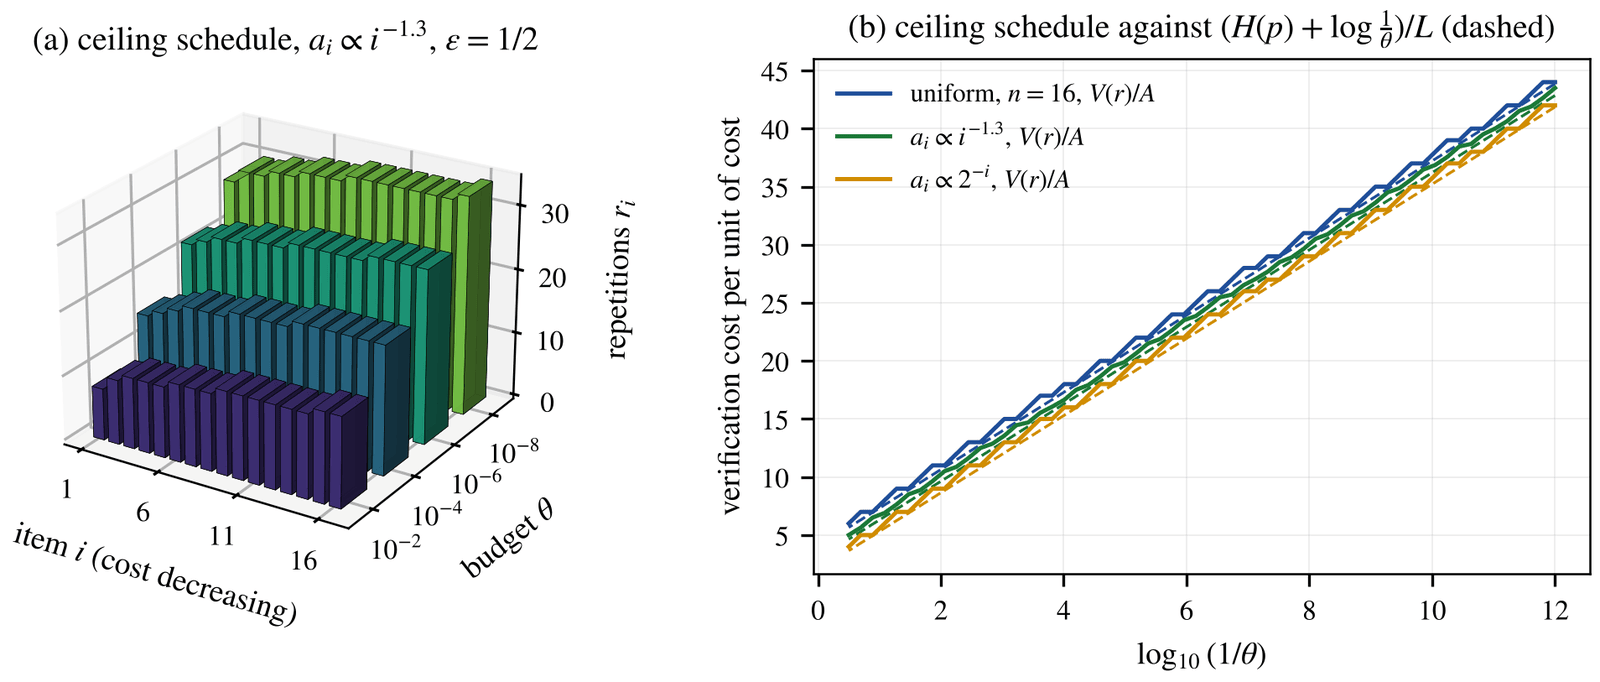
\includegraphics[width=0.98\textwidth]{figures/fig_schedule3d}
\caption{The entropy law. (a) The ceiling schedule $r_{i}=\lceil\log_{2}(A/(\theta a_{i}))\rceil$ for sixteen candidates with costs $a_{i}\propto i^{-1.3}$ and $\eps=\frac12$, at the budgets $\theta=10^{-2}$, $10^{-4}$, $10^{-6}$, $10^{-8}$: the expensive candidates receive the fewest runs, and each factor $100$ of $\theta$ adds six or seven runs to every check. (b) The cost of the ceiling schedule divided by $A$, for the uniform profile on sixteen candidates and the profiles $a_{i}\propto i^{-1.3}$ and $a_{i}\propto2^{-i}$ on sixteen, against the lower bound $(H(p)+\log\frac1\theta)/L$ (dashed). The curves stay in the band of width one above the bound, as Theorem~\ref{thm:A} asserts, and the more skewed the profile the lower the line.}
\label{fig:schedule}
\end{figure*}

\begin{corollary}[Equal costs]\label{cor:uniform}
For $n$ candidates of cost $a$ each, $\frac{na}{L}\log\frac n\theta\le\Vs(\theta)\le\frac{na}{L}\log\frac n\theta+na$. In particular the number of runs per candidate in an optimal schedule is $\log(n/\theta)/L+O(1)$.
\end{corollary}

\begin{proof}
Here $A=na$ and $H(p)=\log n$.
\end{proof}

\begin{proposition}[Shape of the optimum]\label{prop:shape}
Every optimal schedule is antitone in the costs: if $a_{i}>a_{j}$ then $r_{i}\le r_{j}$. The real relaxation, the minimum of $\sum a_{i}x_{i}$ over $x\in[0,\infty)^{n}$ with $\sum\eps^{x_{i}}\le\theta$, is attained only at $x_{i}=\log(A/(\theta a_{i}))/L$ and equals the lower bound of \eqref{eq:entropylaw}.
\end{proposition}

\begin{proof}
If $a_{i}>a_{j}$ and $r_{i}>r_{j}$, exchanging $r_{i}$ and $r_{j}$ keeps $\sum\eps^{r}$ and lowers the cost by $(a_{i}-a_{j})(r_{i}-r_{j})>0$, so $r$ was not optimal. For the relaxation, Proposition~\ref{prop:entropyineq} with $\beta_{i}=\eps^{x_{i}}$ gives $\sum a_{i}x_{i}\ge(A/L)(H+\log\frac1\theta)$, with equality exactly when $\eps^{x_{i}}=\theta p_{i}$.
\end{proof}

The marginal price of soundness is constant: lowering $\theta$ by a factor $e$ raises the lower bound by $A/L$, one nat of soundness bought on every check.

\begin{corollary}[Checks of different soundness]\label{cor:hetero}
If the check of candidate $i$ has soundness $\eps_{i}$, put $L_{i}=\log(1/\eps_{i})$, $b_{i}=a_{i}/L_{i}$, $B=\sum b_{i}$ and $q=b/B$. Then the least cost of a schedule with $\sum\eps_{i}^{r_{i}}\le\theta$, for $0<\theta\le1$, lies between $B(H(q)+\log\frac1\theta)$ and $B(H(q)+\log\frac1\theta)+A$.
\end{corollary}

\begin{proof}
The cost is $\sum a_{i}r_{i}=\sum b_{i}(r_{i}L_{i})$ and $\eps_{i}^{r_{i}}=e^{-r_{i}L_{i}}$. Proposition~\ref{prop:entropyineq} with weights $b_{i}$ and $\beta_{i}=e^{-r_{i}L_{i}}$ gives the lower bound, and $r_{i}=\lceil\log(B/(\theta b_{i}))/L_{i}\rceil$ gives $\sum\eps_{i}^{r_{i}}\le\theta\sum b_{i}/B=\theta$ and cost below $\sum b_{i}\log(B/(\theta b_{i}))+\sum a_{i}$.
\end{proof}

So the right unit of cost is the cost of one nat of soundness, $a_{i}/L_{i}$, and the entropy is that of the profile measured in this unit.

\subsection{Infinitely many candidates}

\begin{proposition}\label{prop:infinite}
Let $(a_{n})_{n\ge1}$ be positive with $A=\sum a_{n}<\infty$, and let $\Vs(\theta)$ be the infimum of $\sum a_{n}r_{n}$ over $r\in\NN^{\NN}$ with $\sum\eps^{r_{n}}\le\theta$. Then \eqref{eq:entropylaw} holds for $0<\theta\le1$, with both sides infinite when $H(p)=\infty$.
\end{proposition}

\begin{proof}
Let $r$ be feasible and $N\ge1$. The first $N$ terms satisfy $\sum_{n\le N}\eps^{r_{n}}\le\theta$, so the finite lower bound gives, with $A_{N}=\sum_{n\le N}a_{n}$ and by \eqref{eq:AH},
\[
\sum_{n\le N}a_{n}\log\frac1{a_{n}}+A_{N}\log A_{N}+A_{N}\log\frac1\theta\le L\sum_{n\le N}a_{n}r_{n}\le L\,V(r).
\]
The terms $a_{n}\log(1/a_{n})$ are positive once $a_{n}<1$, which holds for all large $n$, so as $N\to\infty$ the left side tends to $\sum_{n}a_{n}\log(1/a_{n})+A\log A+A\log(1/\theta)=A(H(p)+\log\frac1\theta)$, finite or infinite. This is the lower bound. The ceiling schedule $r_{n}=\lceil\log(A/(\theta a_{n}))/L\rceil$ satisfies $\sum\eps^{r_{n}}\le\theta\sum p_{n}=\theta$ and $V(r)\le(A/L)(H(p)+\log\frac1\theta)+A$ term by term.
\end{proof}

\subsection{Clean runs}

A stronger requirement than $\EE F\le\theta$ is that the whole run be clean with probability at least $1-\theta$: $\PR_{w}(F=0)\ge1-\theta$ in every world.

\begin{proposition}[Clean runs]\label{prop:clean}
Let $q_{i}=\eps^{r_{i}}$ and $0<\theta<1$. If $\sum q_{i}\le\theta$ then every world has $\PR_{w}(F=0)\ge1-\theta$. If the checks are sharp and every world has $\PR_{w}(F=0)\ge1-\theta$, then $\sum q_{i}\le\log\frac1{1-\theta}\le\frac{\theta}{1-\theta}$. Hence the least cost of a clean schedule lies between $\Vs(\log\frac1{1-\theta})$ and $\Vs(\theta)$, and Theorem~\ref{thm:A} holds for it with $\log\frac1\theta$ in the lower bound replaced by $\log\frac1\theta-\log\frac1{1-\theta}$.
\end{proposition}

\begin{proof}
In world $w$ the candidates are decided independently, so $\PR_{w}(F=0)=\prod_{i\text{ incorrect}}(1-q_{i}')$ with $q_{i}'\le q_{i}$, and this is at least $\prod_{i}(1-q_{i})$. By induction on $n$, $\prod_{i}(1-q_{i})\ge1-\sum_{i}q_{i}$ for $q_{i}\in[0,1]$: the step is $(1-s)(1-q)=1-s-q+sq\ge1-s-q$. This proves the first claim. In the world in which every candidate is incorrect, sharpness gives $1-\theta\le\prod_{i}(1-q_{i})\le\prod_{i}e^{-q_{i}}=e^{-\sum q_{i}}$, so $\sum q_{i}\le\log\frac1{1-\theta}$, and $\log\frac1{1-\theta}=\sum_{k\ge1}\theta^{k}/k\le\theta/(1-\theta)$.
\end{proof}

\subsection{Random schedules}

A schedule may be drawn at random, provided the draw is independent of the checks: the system may toss coins to decide how hard to test, but not look at the results to decide.

\begin{proposition}[Random oblivious schedules]\label{prop:random}
Let $R$ be a random schedule taking finitely many values $r^{(1)},\dots,r^{(m)}$ with probabilities $w_{1},\dots,w_{m}$, independent of the checks, with $\EE\sum_{i}\eps^{R_{i}}\le\theta$. Then $\EE\,V(R)\ge(A/L)(H(p)+\log\frac1\theta)$.
\end{proposition}

\begin{proof}
Let $\bar r=\sum_{j}w_{j}r^{(j)}\in[0,\infty)^{n}$. By the weighted inequality of arithmetic and geometric means, which is Jensen's inequality for the exponential \cite{Jen06}, $\eps^{\bar r_{i}}=\prod_{j}(\eps^{r^{(j)}_{i}})^{w_{j}}\le\sum_{j}w_{j}\eps^{r^{(j)}_{i}}$, so $\sum_{i}\eps^{\bar r_{i}}\le\EE\sum_{i}\eps^{R_{i}}\le\theta$. Proposition~\ref{prop:entropyineq} with $\beta_{i}=\eps^{\bar r_{i}}$ gives $L\sum_{i}a_{i}\bar r_{i}\ge A(H+\log\frac1\theta)$, and $\sum a_{i}\bar r_{i}=\EE\,V(R)$.
\end{proof}

\begin{remark}[Adaptive protocols]\label{rem:adaptive}
The hypothesis that the schedule ignores the outcomes cannot be dropped. Consider the protocol that gives every check $r=\lceil\log(1/\theta)/L\rceil$ runs and halts the whole process, rejecting every later candidate, at the first rejection. In a world with incorrect candidates $i_{1}<i_{2}<\cdots$, the $j$-th of them is kept only if it and the $j-1$ before it are all falsely accepted, which has probability at most $\theta^{j}$, so $\EE_{w}F\le\sum_{j\ge1}\theta^{j}=\theta/(1-\theta)$. Its cost in the world in which every candidate is correct is $Ar<(A/L)\log\frac1\theta+A$, without the entropy term. The saving is paid for elsewhere: a single incorrect candidate stops the process and every correct candidate after it is lost. Theorem~\ref{thm:A} is therefore a theorem about protocols that decide each candidate on its own evidence, which is what a system that must keep its correct work has to do; whether an entropy term returns for adaptive protocols that keep every correct candidate and are charged their worst-case cost is a question we leave open.
\end{remark}

\subsection{Two-sided checks}\label{ssec:twosided}

Learned verifiers err in both directions. Suppose a run of the check of candidate $i$ returns the correct verdict with probability $1-q$ and the wrong one with probability $q<\frac12$, for correct and incorrect candidates alike, and the protocol keeps the candidate when a majority of $r_{i}$ runs, $r_{i}$ odd, accept. Then there are false acceptances and false rejections, and we ask that the expected number of each be at most $\theta$. Write
\[
D=\tfrac12\log\frac1{4q(1-q)}=\mathrm{KL}\bigl(\mathrm{Ber}(\tfrac12)\,\big\|\,\mathrm{Ber}(q)\bigr),
\]
the Chernoff exponent of the majority test \cite{Che52,CT06}.

\begin{proposition}[Two-sided checks]\label{prop:twosided}
\begin{enumerate}[label=\textup{(\roman*)},leftmargin=2.2em,itemsep=1pt]
\item A majority of $r$ runs errs with probability at most $(4q(1-q))^{r/2}=e^{-Dr}$.
\item For $0<\theta\le1$ the schedule $r_{i}$ equal to the least odd integer at least $\log(A/(\theta a_{i}))/D$ has at most $\theta$ expected false acceptances and at most $\theta$ expected false rejections, and costs at most $(A/D)(H(p)+\log\frac1\theta)+2A$.
\item Every decision rule that keeps a candidate whose runs all accept, used with any schedule with at most $\theta$ expected false acceptances in every world, costs at least $(A/\log(1/q))(H(p)+\log\frac1\theta)$.
\end{enumerate}
\end{proposition}

\begin{proof}
(i) Let $S$ be the number of wrong verdicts among $r$ runs, a binomial variable with parameters $r$ and $q$; the majority errs when $S\ge r/2$. For $t>0$, Markov's inequality applied to $e^{tS}$ gives $\PR(S\ge r/2)\le e^{-tr/2}(1-q+qe^{t})^{r}$. With $e^{t}=(1-q)/q>1$ the bracket is $2(1-q)$ and $e^{-tr/2}=(q/(1-q))^{r/2}$, so the bound is $2^{r}(1-q)^{r/2}q^{r/2}=(4q(1-q))^{r/2}$.
(ii) By (i) each candidate is misjudged with probability at most $e^{-Dr_{i}}\le\theta a_{i}/A$, whichever its label, so the expected numbers of both errors are at most $\theta$; and $r_{i}<\log(A/(\theta a_{i}))/D+2$.
(iii) An incorrect candidate whose $r_{i}$ runs all return the wrong verdict is kept, which has probability $q^{r_{i}}$; in the world in which every candidate is incorrect the expected number of false acceptances is at least $\sum q^{r_{i}}$, so $\sum q^{r_{i}}\le\theta$, and Proposition~\ref{prop:entropyineq} with $\beta_{i}=q^{r_{i}}$ gives the bound.
\end{proof}

The rate $D$ is the exact exponent of the majority vote: by the method of types, $\PR(S\ge r/2)\ge(r+1)^{-1}e^{-r\,\mathrm{KL}(\lceil r/2\rceil/r\,\|\,q)}$ \cite{CT06}, and $\mathrm{KL}(\lceil r/2\rceil/r\,\|\,q)\to D$. So for two-sided checks the entropy law holds with $L$ replaced by $D$, and the price of a check that can err in both directions, compared with a one-sided check of the same per-run error $q$, is the ratio $\log(1/q)/D$, which tends to $2$ as $q\to0$ and to infinity as $q\to\frac12$.
